% !TeX program = xelatex
\documentclass[a4paper,10pt]{article}

% ============================================================================
% ១. កញ្ចប់បណ្ណាល័យ និងការកំណត់ទំព័រ (Packages & Page Setup — តាមគំរូ ls_plan.tex)
% ============================================================================
\usepackage[a4paper, left=0.95cm, right=0.95cm, top=0.85cm, bottom=0.92cm, footskip=0.52cm]{geometry}
\usepackage{amsmath}
\usepackage{unicode-math}
\usepackage{fontspec}
\usepackage{longtable, array, multirow, colortbl}
\usepackage[table]{xcolor}
\usepackage{enumitem}
\usepackage{pifont}
\usepackage{fancyhdr}
\usepackage{tikz}
\usetikzlibrary{calc, arrows.meta, decorations.pathreplacing, patterns, positioning, babel}

\makeatletter
\let\@expl@@@mark@update@singlecol@structures@@\relax
\makeatother

% --- ប្រព័ន្ធស្វែងរកទីតាំងពុម្ពអក្សរស្វ័យប្រវត្តិ (Windows Local + Cloud Repo fonts/) ---
\providecommand{\NGSFindFonts}{%
  \IfFileExists{C:/Windows/Fonts/cambria.ttc}{%
    \def\NGSSysPath{C:/Windows/Fonts/}%
    \def\NGSUserPath{C:/Users/KIT/AppData/Local/Microsoft/Windows/Fonts/}%
  }{%
    \IfFileExists{./fonts/KhmerOSsiemreap.ttf}{\def\NGSSysPath{./fonts/}\def\NGSUserPath{./fonts/}}{%
    \IfFileExists{../fonts/KhmerOSsiemreap.ttf}{\def\NGSSysPath{../fonts/}\def\NGSUserPath{../fonts/}}{%
    \IfFileExists{../../fonts/KhmerOSsiemreap.ttf}{\def\NGSSysPath{../../fonts/}\def\NGSUserPath{../../fonts/}}{%
    \IfFileExists{../../../fonts/KhmerOSsiemreap.ttf}{\def\NGSSysPath{../../../fonts/}\def\NGSUserPath{../../../fonts/}}{%
    \IfFileExists{../../../../fonts/KhmerOSsiemreap.ttf}{\def\NGSSysPath{../../../../fonts/}\def\NGSUserPath{../../../../fonts/}}{%
    \IfFileExists{../../../../../fonts/KhmerOSsiemreap.ttf}{\def\NGSSysPath{../../../../../fonts/}\def\NGSUserPath{../../../../../fonts/}}{%
    \IfFileExists{../../../../../../fonts/KhmerOSsiemreap.ttf}{\def\NGSSysPath{../../../../../../fonts/}\def\NGSUserPath{../../../../../../fonts/}}{%
      \def\NGSSysPath{../../../../../../../fonts/}\def\NGSUserPath{../../../../../../../fonts/}%
    }}}}}}}%
  }%
}
\NGSFindFonts

% ============================================================================
% ២. កំណត់ពុម្ពអក្សរ (Fonts — តាមគំរូ ls_plan.tex)
% ============================================================================
\setmathfont[Path={\NGSSysPath}, FontIndex=1, Scale=1.02]{cambria.ttc}
\defaultfontfeatures{Ligatures=TeX}

\setmainfont[
  Path={\NGSUserPath},
  Extension=.ttf,
  Script=Khmer,
  BoldFont={KhmerOSsiemreap},
  BoldFeatures={FakeBold=1.8},
  ItalicFont={KhmerOSsiemreap},
  ItalicFeatures={FakeSlant=0.25},
  BoldItalicFont={KhmerOSsiemreap},
  BoldItalicFeatures={FakeBold=1.8, FakeSlant=0.25}
]{KhmerOSsiemreap}

\newfontfamily\muol[Path={\NGSUserPath}, Extension=.ttf, Script=Khmer]{KhmerOSmuollight}
\newfontfamily\Tacteing[Path={\NGSUserPath}, Extension=.TTF]{TACTENG}
\newfontfamily\TimesEn[Path={\NGSSysPath}, Extension=.ttf, BoldFont={timesbd}, ItalicFont={timesi}, BoldItalicFont={timesbi}]{times}
\newfontfamily\CalibriFont[Path={\NGSSysPath}, Extension=.ttf]{calibri}
\newfontfamily\CourierCirc[Path={\NGSSysPath}, Extension=.ttf]{cour}

\XeTeXlinebreaklocale "km"
\XeTeXlinebreakskip = 0pt plus 1pt minus 0.1pt

% ============================================================================
% ៣. ពណ៌ និងការតុបតែង (Colors & Styles)
% ============================================================================
\definecolor{stepbg}{HTML}{D9D9D9}
\definecolor{headgray}{HTML}{E6E6E6}
\definecolor{emphred}{HTML}{C00000}

\pagestyle{fancy}
\fancyhf{}
\renewcommand{\headrulewidth}{0pt}
\fancyfoot[R]{\CalibriFont\fontsize{9pt}{11pt}\selectfont\thepage}

\setlength{\parindent}{0pt}
\setlength{\parskip}{0pt}
\setlength{\tabcolsep}{4.5pt}
\setlength{\LTpre}{2pt}
\setlength{\LTpost}{2pt}

\newcolumntype{L}[1]{>{\raggedright\arraybackslash}p{#1}}
\newcolumntype{C}[1]{>{\centering\arraybackslash}p{#1}}

% ============================================================================
% ៤. ពាក្យបញ្ជាជំនួយ (Helper Macros)
% ============================================================================
\newcommand{\en}[1]{{\TimesEn #1}}
\newcommand{\enbf}[1]{{\TimesEn\bfseries #1}}
\newcommand{\khmflourish}{{\Tacteing\fontsize{15pt}{15pt}\selectfont 3}}
\newcommand{\wcirc}{{\CourierCirc\fontsize{9.5pt}{11pt}\selectfont o}}
\newcommand{\ditem}{{\fontsize{7.5pt}{10pt}\selectfont\ding{117}}\ }
\newcommand{\fiveE}[1]{\textcolor{emphred}{\CalibriFont\bfseries #1}}
\newcommand{\redsub}[1]{\textcolor{emphred}{#1}}
\newcommand{\timenote}[1]{\textcolor{emphred}{\textit{#1}}}
\newcommand{\stepheader}[1]{\multicolumn{3}{|c|}{\cellcolor{stepbg}\muol #1} \\ \hline}
\newcommand{\cfig}[1]{{\centering\vspace{3pt}#1\vspace{3pt}\par}}
\newcommand{\cnum}[1]{\mbox{\fontsize{10.5pt}{12pt}\selectfont\ding{\numexpr181+#1\relax}}}
\newcommand{\unit}[1]{\,\text{\en{#1}}}
\newcommand{\riel}{\,\text{៛}}
\newcommand{\usd}{\,\text{\en{\$}}}
\newcommand{\graybox}[1]{\colorbox{headgray}{\strut #1}}

% ============================================================================
% ៥. រូបភាព TikZ ស-ខ្មៅ សម្រាប់បង្រៀនលើក្ដារខៀន និងសន្លឹកកិច្ចការ (B&W Diagrams)
% ============================================================================

% ១. E1 Engage: កុងត្រាខ្ចីប្រាក់ 1 000 000៛ អត្រា 12%/ឆ្នាំ រយៈពេល 6 ខែ
\newcommand{\figEngageINTThreeTwoFive}{%
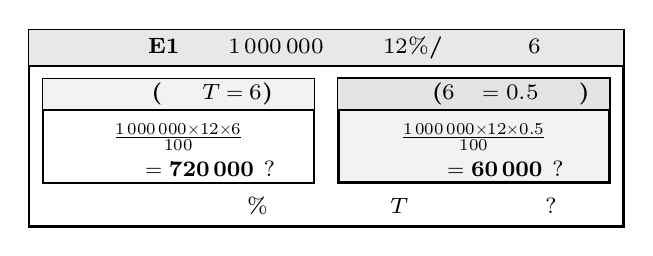
\begin{tikzpicture}[x=1cm, y=1cm, every node/.style={font=\footnotesize, text=black}]
  \draw[black, line width=0.9pt] (0,0) rectangle (7.55,2.50);
  \fill[gray!18] (0,2.04) rectangle (7.55,2.50);
  \draw[black, line width=0.6pt] (0,2.04) -- (7.55,2.04);
  \node at (3.775,2.27) {\textbf{បេសកកម្ម \en{E1}៖ ខ្ចី $1\,000\,000\riel$ អត្រា $12\%$/ឆ្នាំ រយៈពេល $6$ ខែ}};

  % Left: Sok
  \draw[black, line width=0.8pt] (0.18,0.56) rectangle (3.62,1.88);
  \fill[gray!10] (0.18,1.48) rectangle (3.62,1.88);
  \draw[black, line width=0.5pt] (0.18,1.48) -- (3.62,1.48);
  \node at (1.90,1.68) {\textbf{ស្មៀន សុខ (ជំនួស $T = 6$)}};
  \node at (1.90,1.14) {$\tfrac{1\,000\,000\times 12\times 6}{100}$};
  \node at (1.90,0.74) {ការប្រាក់ $= \mathbf{720\,000\riel}$?};

  % Right: Dara
  \draw[black, line width=0.95pt, fill=gray!10] (3.93,0.56) rectangle (7.37,1.88);
  \fill[gray!22] (3.93,1.48) rectangle (7.37,1.88);
  \draw[black, line width=0.55pt] (3.93,1.48) -- (7.37,1.48);
  \node at (5.65,1.68) {\textbf{ស្មៀន តារា ($6\text{ ខែ} = 0.5\text{ ឆ្នាំ}$)}};
  \node at (5.65,1.14) {$\tfrac{1\,000\,000\times 12\times 0.5}{100}$};
  \node at (5.65,0.74) {ការប្រាក់ $= \mathbf{60\,000\riel}$?};

  \node at (3.775,0.26) {\textbf{សំណួរគន្លឹះ៖} ពេលអត្រាជា $\%$ \textbf{ក្នុង ១ ឆ្នាំ} តើ $T$ ត្រូវគិតជា\textbf{ខែ} ឬជា\textbf{ឆ្នាំ}?};
\end{tikzpicture}}

% ២. E2 Explore: បន្ទាត់ពេលវេលាកើនការប្រាក់ថេរប្រចាំឆ្នាំរបស់ពូសំ (ទំ.៣៦)
\newcommand{\figTimelineINTThreeTwoFive}{%
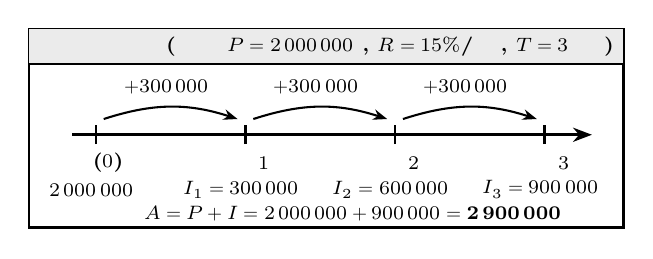
\begin{tikzpicture}[x=1cm, y=1cm, every node/.style={font=\scriptsize, text=black}]
  \draw[black, line width=0.9pt] (0,0) rectangle (7.55,2.52);
  \fill[gray!16] (0,2.08) rectangle (7.55,2.52);
  \draw[black, line width=0.6pt] (0,2.08) -- (7.55,2.08);
  \node at (3.775,2.30) {\textbf{បន្ទាត់កើនការប្រាក់ថេរ (ពូសំខ្ចី $P = 2\,000\,000\riel$, $R = 15\%$/ឆ្នាំ, $T = 3$ ឆ្នាំ)}};

  % Timeline axis
  \draw[-{Stealth[length=2.4mm]}, black, line width=1.0pt] (0.55,1.18) -- (7.15,1.18);
  \foreach \x/\yr/\tot in {0.85/ដើម ($0$)/$2\,000\,000\riel$, 2.75/ឆ្នាំទី$1$/$I_1=300\,000\riel$, 4.65/ឆ្នាំទី$2$/$I_2=600\,000\riel$, 6.55/ឆ្នាំទី$3$/$I_3=900\,000\riel$} {
    \draw[black, line width=0.9pt] (\x,1.06) -- (\x,1.30);
    \node at (\x,0.82) {\textbf{\yr}};
    \node at (\x,0.48) {\tot};
  }
  % Equal jumps
  \draw[-{Stealth[length=1.8mm]}, black, line width=0.75pt] (0.95,1.38) to[bend left=18] node[above=1pt] {$+300\,000\riel$} (2.65,1.38);
  \draw[-{Stealth[length=1.8mm]}, black, line width=0.75pt] (2.85,1.38) to[bend left=18] node[above=1pt] {$+300\,000\riel$} (4.55,1.38);
  \draw[-{Stealth[length=1.8mm]}, black, line width=0.75pt] (4.75,1.38) to[bend left=18] node[above=1pt] {$+300\,000\riel$} (6.45,1.38);

  \node at (3.775,0.18) {ប្រាក់សរុប $A = P + I = 2\,000\,000 + 900\,000 = \mathbf{2\,900\,000\riel}$};
\end{tikzpicture}}

% ៣. E3 Explain: ប្រអប់អថេរ P-R-T-I-A និងច្រកត្រួតពិនិត្យឯកតា (Schema & Unit Gate)
\newcommand{\figSchemaGateINTThreeTwoFive}{%
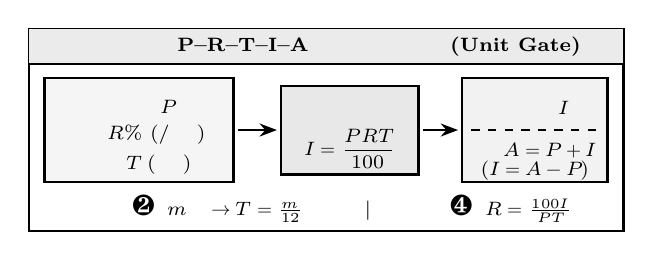
\begin{tikzpicture}[x=1cm, y=1cm, every node/.style={font=\scriptsize, text=black}]
  \draw[black, line width=0.9pt] (0,0) rectangle (7.55,2.56);
  \fill[gray!16] (0,2.12) rectangle (7.55,2.56);
  \draw[black, line width=0.6pt] (0,2.12) -- (7.55,2.12);
  \node at (3.775,2.34) {\textbf{ប្រព័ន្ធប្រអប់អថេរ \en{P--R--T--I--A} និងច្រកត្រួតពិនិត្យឯកតា (\en{Unit Gate})}};

  % Left: Inputs P, R, T
  \draw[black, line width=0.85pt, fill=gray!8] (0.20,0.62) rectangle (2.60,1.94);
  \node[align=left] at (1.40,1.58) {\textbf{ប្រាក់ដើម} $P$};
  \node[align=left] at (1.40,1.22) {\textbf{អត្រា} $R\%$ (/ឆ្នាំ)};
  \node[align=left] at (1.40,0.84) {\textbf{រយៈពេល} $T$ (\textbf{ឆ្នាំ})};

  % Arrow to center formula
  \draw[-{Stealth[length=2.2mm]}, black, line width=0.9pt] (2.65,1.28) -- (3.15,1.28);

  % Center formula box
  \draw[black, line width=1.0pt, fill=gray!18] (3.20,0.72) rectangle (4.95,1.84);
  \node at (4.075,1.52) {\textbf{រូបមន្តគោល}};
  \node at (4.075,1.04) {$I = \dfrac{PRT}{100}$};

  % Arrow to right outputs I, A
  \draw[-{Stealth[length=2.2mm]}, black, line width=0.9pt] (5.00,1.28) -- (5.45,1.28);

  % Right: Outputs I, A
  \draw[black, line width=0.95pt, fill=gray!10] (5.50,0.62) rectangle (7.35,1.94);
  \node at (6.425,1.56) {\textbf{ការប្រាក់} $I$};
  \draw[black, dashed, line width=0.5pt] (5.62,1.28) -- (7.23,1.28);
  \node at (6.425,1.02) {\textbf{សរុប} $A = P + I$};
  \node at (6.425,0.76) {($I = A - P$)};

  % Bottom gate
  \node at (3.775,0.28) {\textbf{ច្រកឯកតា \cnum{2}៖} $m\text{ ខែ} \to T = \tfrac{m}{12}\text{ ឆ្នាំ}$ \quad \en{|} \quad \textbf{បញ្ច្រាស \cnum{4}៖} $R = \tfrac{100I}{PT}$};
\end{tikzpicture}}

% ៤. E4 Elaborate: ប្រៀបធៀបលំហាត់គំរូមីងថន (ទំ.៣៦ ក និង ខ)
\newcommand{\figElaborateThonINTThreeTwoFive}{%
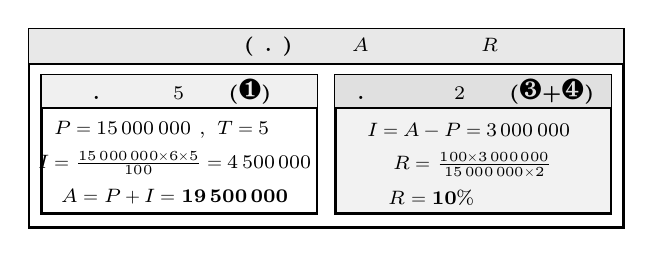
\begin{tikzpicture}[x=1cm, y=1cm, every node/.style={font=\scriptsize, text=black}]
  \draw[black, line width=0.9pt] (0,0) rectangle (7.55,2.52);
  \fill[gray!18] (0,2.08) rectangle (7.55,2.52);
  \draw[black, line width=0.6pt] (0,2.08) -- (7.55,2.08);
  \node at (3.775,2.30) {\textbf{លំហាត់គំរូមីងថន (ទំ.៣៦)៖ ទៅមុខរក $A$ ទល់នឹង បញ្ច្រាសរក $R$}};

  % Left: Part ក
  \draw[black, line width=0.8pt] (0.16,0.18) rectangle (3.66,1.94);
  \fill[gray!12] (0.16,1.52) rectangle (3.66,1.94);
  \draw[black, line width=0.55pt] (0.16,1.52) -- (3.66,1.52);
  \node at (1.91,1.73) {\textbf{ក. ផ្ញើធនាគារ $5$ ឆ្នាំ (\cnum{1})}};
  \node at (1.91,1.24) {$P = 15\,000\,000\riel, \ T = 5\text{ ឆ្នាំ}$};
  \node at (1.91,0.82) {$I = \tfrac{15\,000\,000\times 6\times 5}{100} = 4\,500\,000\riel$};
  \node at (1.91,0.40) {$A = P + I = \mathbf{19\,500\,000\riel}$};

  % Right: Part ខ
  \draw[black, line width=0.95pt, fill=gray!10] (3.89,0.18) rectangle (7.39,1.94);
  \fill[gray!24] (3.89,1.52) rectangle (7.39,1.94);
  \draw[black, line width=0.6pt] (3.89,1.52) -- (7.39,1.52);
  \node at (5.64,1.73) {\textbf{ខ. ឱ្យមីងសានខ្ចី $2$ ឆ្នាំ (\cnum{3}+\cnum{4})}};
  \node at (5.64,1.24) {$I = A - P = 3\,000\,000\riel$};
  \node at (5.64,0.80) {$R = \tfrac{100\times 3\,000\,000}{15\,000\,000\times 2}$};
  \node at (5.64,0.38) {$R = \mathbf{10\%}\text{ ក្នុង ១ ឆ្នាំ}$};
\end{tikzpicture}}

% ៥. E5 Evaluate: ជម្រើសវិនិច្ឆ័យ A-D (ខ្ចី 4 000 000៛ អត្រា 9%/ឆ្នាំ រយៈពេល 8 ខែ រកការប្រាក់ I)
\newcommand{\figExitINTThreeTwoFive}{%
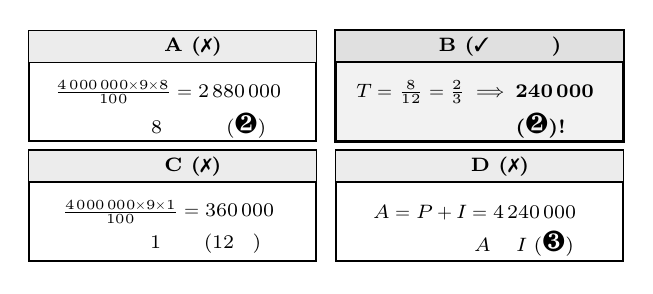
\begin{tikzpicture}[x=1cm, y=1cm, every node/.style={font=\scriptsize, text=black}]
  % A
  \draw[black, line width=0.8pt] (0,1.52) rectangle (3.65,2.92);
  \fill[gray!15] (0,2.52) rectangle (3.65,2.92);
  \draw[black, line width=0.55pt] (0,2.52) -- (3.65,2.52);
  \node at (1.825,2.72) {\textbf{ជម្រើស \en{A} (\ding{55})}};
  \node at (1.825,2.14) {$\tfrac{4\,000\,000\times 9\times 8}{100} = 2\,880\,000\riel$};
  \node at (1.825,1.72) {ភ្លេចបំប្លែង $8$ ខែជាឆ្នាំ (\cnum{2})};

  % B (Correct)
  \draw[black, line width=1.1pt, fill=gray!10] (3.90,1.52) rectangle (7.55,2.92);
  \fill[gray!24] (3.90,2.52) rectangle (7.55,2.92);
  \draw[black, line width=0.6pt] (3.90,2.52) -- (7.55,2.52);
  \node at (5.725,2.72) {\textbf{ជម្រើស \en{B} (\ding{51} ត្រឹមត្រូវ)}};
  \node at (5.725,2.14) {$T = \tfrac{8}{12} = \tfrac{2}{3}\implies \mathbf{240\,000\riel}$};
  \node at (5.725,1.72) {\textbf{ឯកតាឆ្នាំត្រូវគ្នាគត់ (\cnum{2})!}};

  % C
  \draw[black, line width=0.8pt] (0,0) rectangle (3.65,1.40);
  \fill[gray!15] (0,1.00) rectangle (3.65,1.40);
  \draw[black, line width=0.55pt] (0,1.00) -- (3.65,1.00);
  \node at (1.825,1.20) {\textbf{ជម្រើស \en{C} (\ding{55})}};
  \node at (1.825,0.62) {$\tfrac{4\,000\,000\times 9\times 1}{100} = 360\,000\riel$};
  \node at (1.825,0.22) {ច្រឡំគិតពេញ $1$ ឆ្នាំ ($12$ ខែ)};

  % D
  \draw[black, line width=0.8pt] (3.90,0) rectangle (7.55,1.40);
  \fill[gray!15] (3.90,1.00) rectangle (7.55,1.40);
  \draw[black, line width=0.55pt] (3.90,1.00) -- (7.55,1.00);
  \node at (5.725,1.20) {\textbf{ជម្រើស \en{D} (\ding{55})}};
  \node at (5.725,0.62) {$A = P + I = 4\,240\,000\riel$};
  \node at (5.725,0.22) {ច្រឡំប្រាក់សរុប $A$ ជា $I$ (\cnum{3})};
\end{tikzpicture}}

% ============================================================================
% ចាប់ផ្ដើមឯកសារ (Document Body)
% ============================================================================
\begin{document}
\fontsize{10pt}{15.2pt}\selectfont

% -------------------- ក្បាលកិច្ចតែងការ (Header) --------------------
\begin{center}
  {\muol\fontsize{11pt}{16pt}\selectfont ព្រះរាជាណាចក្រកម្ពុជា}\\[2pt]
  {\muol\fontsize{10pt}{15pt}\selectfont ជាតិ សាសនា ព្រះមហាក្សត្រ}\\[1pt]
  \khmflourish
\end{center}

\vspace{-24pt}
{\muol\fontsize{9.5pt}{12.5pt}\selectfont
មន្ទីរអប់រំ យុវជន និងកីឡា ខេត្តកំពង់ធំ\\
ការិយាល័យអប់រំ យុវជន និងកីឡា ស្រុកកំពង់ស្វាយ\\
អនុវិទ្យាល័យព្រះក្រសាំង}

\vspace{1pt}
\begin{center}
  {\muol\fontsize{10pt}{14pt}\selectfont កិច្ចតែងការបង្រៀន}
\end{center}
\vspace{0pt}

% -------------------- ព័ត៌មានទូទៅ (Metadata) --------------------
{\renewcommand{\arraystretch}{0.98}
\hspace*{3.1cm}%
\begin{tabular}{@{}l l L{11.0cm}@{}}
  - \hspace{0.35cm} មុខវិជ្ជា & : & គណិតវិទ្យា ថ្នាក់ទី៨ (ពីជគណិត) \\
  - \hspace{0.35cm} ចំណងជើងមេរៀន & : & មេរៀនទី៣៖ ទំហំសមាមាត្រនិងភាគរយ \\
  - \hspace{0.35cm} ចំណងជើងរង & : & ២.៥. ការប្រាក់សាមញ្ញ (ទំ.៣៥–៣៧, ៤២) \\
  - \hspace{0.35cm} រយៈពេល & : & ១ ម៉ោងសិក្សា (៥០ នាទី) \\
  - \hspace{0.35cm} បង្រៀនដោយ & : & ហុក ប៊ុនថែន \\
  - \hspace{0.35cm} កាលបរិច្ឆេទ & : & ថ្ងៃអង្គារ ទី២៤ ខែវិច្ឆិកា ឆ្នាំ២០២៦ \\
\end{tabular}

\vspace{2pt}

% -------------------- I. វត្ថុបំណង --------------------
\textbf{I.} {\muol វត្ថុបំណង}\\[1pt]
\hspace*{0.45cm}%
\begin{tabular}{@{}l l L{14.85cm}@{}}
  \wcirc \hspace{0.25cm} វិជ្ជាសម្បទា & : & សិស្សប្រាប់និយមន័យនៃការប្រាក់ ($I$) ប្រាក់ដើម ($P$) អត្រាការប្រាក់ក្នុងមួយឆ្នាំ ($R\%$) រយៈពេល ($T$) ប្រាក់សរុប ($A = P + I$) និងរូបមន្តការប្រាក់សាមញ្ញ $I = \frac{PRT}{100}$ ព្រមទាំងរូបមន្តបញ្ច្រាសបានត្រឹមត្រូវ ។ \\
  \wcirc \hspace{0.25cm} បំណិនសម្បទា & : & សិស្សគណនាការប្រាក់សាមញ្ញ ប្រាក់សរុប អត្រាការប្រាក់ និងប្រាក់ដើម (រួមទាំងការបំប្លែងខែជាឆ្នាំ $T = \frac{m}{12}$) តាមប្រអប់អថេរ \en{P--R--T--I--A} លើសន្លឹកកិច្ចការបានត្រឹមត្រូវ ។ \\
  \wcirc \hspace{0.25cm} ចរិយាសម្បទា & : & សិស្សមានទម្លាប់ពិនិត្យឯកតាអត្រានិងរយៈពេលក្នុងកិច្ចសន្យាសន្សំឬខ្ចីប្រាក់ដោយប្រុងប្រយ័ត្ន និងយល់តម្លៃនៃការសន្សំប្រាក់ក្នុងគ្រួសារ ។ \\
\end{tabular}

\vspace{2pt}

% -------------------- II. សម្ភារៈឧបទេស --------------------
\textbf{II.} {\muol សម្ភារៈឧបទេស}\\[1pt]
\hspace*{0.55cm}$\bullet$ \hspace{0.35cm} សៀវភៅសិក្សាគោលថ្នាក់ទី៨ (ទំ.៣៥–៣៧, ៤២) ក្ដារខៀន ដីស/ហ្វឺត បន្ទាត់ត្រង់ និង\textbf{សន្លឹកកិច្ចការសិស្សបំពេញចន្លោះ ស-ខ្មៅ} (\en{Printable\_Materials\_INT325} ទំព័រ ១–២ សម្រាប់សិស្ស និងទំព័រ ៣ ប្លង់ក្ដារខៀន/ចម្លើយគ្រូ — គ្មានប្រើ \en{LCD})

\vspace{2pt}

% -------------------- III. វិធីសាស្រ្តបង្រៀន --------------------
\textbf{III.} {\muol វិធីសាស្រ្តបង្រៀន}\\[1pt]
\hspace*{0.45cm}%
\begin{tabular}{@{}l l L{14.85cm}@{}}
  $\bullet$ \hspace{0.25cm} គោលវិធី & : & សិស្សមជ្ឈមណ្ឌល (សន្លឹកកិច្ចការបំពេញចន្លោះជាគោល + ការពិភាក្សាជាក្រុមតូច ៣ នាក់) \\
  $\bullet$ \hspace{0.25cm} យុទ្ធវិធីបង្រៀន & : & គំរូស្ថាបនានិយម \en{5Es} រួមបញ្ចូល \textbf{បន្ទាត់កើនការប្រាក់ថេរប្រចាំឆ្នាំ (\en{Linear Accrual})} និង \textbf{ប្រអប់អថេរ \en{P--R--T--I--A} ភ្ជាប់ច្រកឯកតាពេលវេលា} \\
\end{tabular}
}

\vspace{2pt}

% -------------------- IV. ដំណើរការបង្រៀន --------------------
\textbf{IV.} {\muol ដំណើរការបង្រៀន}

\vspace{1pt}
{\renewcommand{\arraystretch}{1.12}
\begin{longtable}{|L{5.50cm}|L{7.90cm}|L{4.80cm}|}
\hline
\multicolumn{1}{|c|}{\cellcolor{headgray}\muol សកម្មភាពគ្រូ} &
\multicolumn{1}{c|}{\cellcolor{headgray}\muol ខ្លឹមសារមេរៀន} &
\multicolumn{1}{c|}{\cellcolor{headgray}\muol សកម្មភាពសិស្ស} \\
\endhead
\hline
\endfoot

% ==================== ជំហានទី១ (2min) ====================
\stepheader{ជំហានទី១ \enbf{(}រដ្ឋបាលថ្នាក់\enbf{)}}
$\bullet$ ពិនិត្យវត្តមាន អនាម័យ និងសណ្ដាប់ធ្នាប់ថ្នាក់រៀន \par
$\bullet$ រៀបចំក្រុមតូច ៣ នាក់តាមតុ និងចែក\textbf{សន្លឹកកិច្ចការសិស្ស (\en{INT325} ទំព័រ ១–២)}
&
$\bullet$ រដ្ឋបាលថ្នាក់ អនាម័យ និងវិន័យសិក្សា \par
$\bullet$ ចែកសន្លឹកកិច្ចការម្នាក់ ១ សន្លឹក សម្រាប់បំពេញតាមដំណាក់កាល \en{E1--E5}
&
$\circ$ ប្រធានថ្នាក់រាយការណ៍វត្តមានសិស្ស \par
$\circ$ ទទួលសន្លឹកកិច្ចការ សរសេរឈ្មោះ និងអង្គុយតាមក្រុម ៣ នាក់ \\
\hline

% ==================== ជំហានទី២ (9min: កំណែ <=3m + រំលឹក 3m + E1 3m) ====================
\stepheader{ជំហានទី២ \enbf{(}កិច្ចការផ្ទះ \enbf{+} ទំនាក់ទំនងមេរៀនថ្មី\enbf{)}}
\ditem \textbf{កំណែកិច្ចការផ្ទះ ($\le\text{\enbf{3\,min}}$)} \par
$\bullet$ ហៅសិស្ស ២ នាក់ឡើងកែប្រតិបត្តិទំ.៣៤ និងលំហាត់ \#14(ខ) ទំ.៤២ លើក្ដារខៀន
&
{\centering\redsub{កំណែកិច្ចការផ្ទះមេរៀនមុន (ប្រតិបត្តិទំ.៣៤ និង ទំ.៤២ \#14 ខ)}\par}
$\bullet$ \textbf{ប្រតិបត្តិ (ទំ.៣៤)៖} ដើម $990\,000\riel$, លក់សរុប $796\,000 + 338\,300 = 1\,134\,300\riel \implies$ ចំណេញ $144\,300\riel$ ត្រូវជា $\mathbf{14.58\%}$ \par
$\bullet$ \textbf{\#14 ខ (ទំ.៤២)៖} សៀវភៅកើន $243 + 63 = 306$ ក្បាល; តម្លៃសៀវភៅថ្មីសរុប $\mathbf{1\,964\,250\riel}$ និងភាគរយកើនសរុប $\frac{306}{4\,500}\times 100\% = \mathbf{6.8\%}$
&
$\circ$ ផ្ទៀងចម្លើយ និងកែតម្រូវចូលសៀវភៅកិច្ចការផ្ទះ \\[3pt]

\ditem \textbf{រំលឹកមេរៀនទាក់ទង (\enbf{3min})} \par
$\bullet$ សួររំលឹក៖ «តើ $15\%$ នៃប្រាក់ $2\,000\,000\riel$ ស្មើប៉ុន្មានរៀល?»
&
{\centering\redsub{រំលឹកការគណនាភាគរយនៃចំនួនមួយ}\par}
$\bullet$ $15\%$ នៃ $2\,000\,000\riel = \dfrac{15}{100}\times 2\,000\,000 = \mathbf{300\,000\riel}$ ។
&
$\circ$ គណនារហ័សឆ្លើយ៖ «ស្មើ $300\,000\riel$!» \\[3pt]

\fiveE{E1 - Engage (3min)} \timenote{(កុំទាន់ផ្ដល់ចម្លើយ)} \par
\ditem \textbf{បេសកកម្មកុងត្រាខ្ចីប្រាក់ ៦ ខែ (សន្លឹកកិច្ចការ \en{E1})} \par
$\bullet$ ឱ្យសិស្សអានប្រអប់ \en{E1} ហើយគូសជ្រើសរើសរវាង\textbf{ស្មៀន សុខ ($720\,000\riel$)} និង\textbf{ស្មៀន តារា ($60\,000\riel$)}
&
\redsub{បេសកកម្ម \en{E1}៖ ខ្ចីប្រាក់កសិកម្ម $1\,000\,000\riel$ រយៈពេល $6$ ខែ} \par
សហគមន៍កសិកម្មឱ្យកសិករម្នាក់ខ្ចីប្រាក់ $1\,000\,000\riel$ ដោយអត្រាការប្រាក់ \textbf{$12\%$ ក្នុង ១ ឆ្នាំ} រយៈពេល \textbf{$6$ ខែ} ។ \par
$\bullet$ ស្មៀនសុខគិតការប្រាក់ $720\,000\riel$ រីឯស្មៀនតារាគិតតែ $60\,000\riel$! តើអ្នកណាគណនាត្រឹមត្រូវ?
&
$\circ$ ពិភាក្សាជាគូ និងគូស \ding{51} ក្នុងប្រអប់ \en{E1} លើសន្លឹកកិច្ចការ \\[3pt]

&
\cfig{\figEngageINTThreeTwoFive}
& \\
\hline

% ==================== ជំហានទី៣ (17min: E2 11m + E3 6m) ====================
\stepheader{ជំហានទី៣ \enbf{(}ខ្លឹមសារមេរៀនថ្មី\enbf{)}}
\fiveE{E2 - Explore (11min)} \par
$\bullet$ សរសេរចំណងជើងរង \textbf{២.៥. ការប្រាក់សាមញ្ញ} លើក្ដារខៀន \par
\ditem \textbf{សកម្មភាព ១៖ បន្ទាត់កើនការប្រាក់ថេររបស់ពូសំ (\enbf{6min}, សន្លឹកកិច្ចការ \en{E2-A})} \par
$\bullet$ ឱ្យសិស្សបំពេញតារាងការប្រាក់ឆ្នាំទី១ ដល់ទី៣ នៃឧទាហរណ៍ពូសំ (សៀវភៅទំ.៣៦)
&
មេរៀនទី៣ \quad {\muol ទំហំសមាមាត្រនិងភាគរយ \enbf{(}ត\enbf{)}} \par
២.៥. ការប្រាក់សាមញ្ញ \par
$\bullet$ \textbf{ឧទាហរណ៍ (ទំ.៣៦ — ពូសំខ្ចីប្រាក់ធនាគារ)៖} \par
ប្រាក់ដើម $P = 2\,000\,000\riel$, អត្រា $R = 15\%$/ឆ្នាំ, រយៈពេល $T = 3$ ឆ្នាំ ៖ \par
\hspace*{0.2cm}-- ការប្រាក់ $1$ ឆ្នាំ $= 2\,000\,000\times \dfrac{15}{100} = 300\,000\riel$ \par
\hspace*{0.2cm}-- ការប្រាក់ $3$ ឆ្នាំ ($I$) $= 300\,000\times 3 = \mathbf{900\,000\riel}$ \par
\hspace*{0.2cm}-- ប្រាក់សរុប ($A = P + I$) $= 2\,000\,000 + 900\,000 = \mathbf{2\,900\,000\riel}$
&
$\circ$ បំពេញតារាងឆ្នាំទី១–ទី៣ លើសន្លឹកកិច្ចការ \en{E2-A} ឃើញការប្រាក់កើនថេរ $300\,000\riel$ ក្នុង ១ ឆ្នាំ \\[3pt]

&
\cfig{\figTimelineINTThreeTwoFive}
& \\[3pt]

\ditem \textbf{សកម្មភាព ២៖ ច្រកត្រួតពិនិត្យឯកតាពេលវេលា (\enbf{5min}, សន្លឹកកិច្ចការ \en{E2-B})} \par
$\bullet$ ឱ្យសិស្សបំប្លែងខែទៅជាឆ្នាំ ($6$ ខែ, $9$ ខែ, $18$ ខែ) តាមកំណត់សម្គាល់សៀវភៅទំ.៣៥
&
$\bullet$ \textbf{ច្រកត្រួតពិនិត្យឯកតា (ទំ.៣៥)៖} \par
បើអត្រាការប្រាក់ $R$ គិតជា \textbf{ភាគរយក្នុង ១ ឆ្នាំ} នោះរយៈពេល $T$ ត្រូវគិតជា\textbf{ឆ្នាំ}ដូចគ្នា ($1\text{ ឆ្នាំ} = 12\text{ ខែ}$) ៖ \par
\hspace*{0.2cm}-- $6\text{ ខែ} = \frac{6}{12} = \mathbf{0.5\text{ ឆ្នាំ}}$; \quad $9\text{ ខែ} = \frac{9}{12} = \mathbf{\frac{3}{4}\text{ ឆ្នាំ}}$; \quad $18\text{ ខែ} = \frac{18}{12} = \mathbf{1.5\text{ ឆ្នាំ}}$
&
$\circ$ បំប្លែងចំនួនខែជាប្រភាគនៃឆ្នាំ ($T = \frac{m}{12}$) លើសន្លឹកកិច្ចការ \en{E2-B} \\[3pt]

% --- E3 Explain (6min) ---
\fiveE{E3 - Explain (6min)} \par
$\bullet$ ដឹកនាំសិស្សទាញរូបមន្ត\textbf{ការប្រាក់សាមញ្ញ} និង\textbf{ប្រាក់សរុប} (ទំ.៣៥–៣៦)
&
$\bullet$ \textbf{និយមន័យ និងរូបមន្តការប្រាក់សាមញ្ញ (ទំ.៣៥–៣៦)៖} \par
តាង $P$ ប្រាក់ដើម, $R\%$ អត្រាការប្រាក់ក្នុង ១ ឆ្នាំ, $T$ រយៈពេល (ឆ្នាំ), $I$ ការប្រាក់សាមញ្ញ និង $A$ ប្រាក់សរុប៖ \par
\hspace*{0.15cm}\graybox{$I = \dfrac{PRT}{100}$} \quad និង \quad \graybox{$A = P + I \iff I = A - P$}
&
$\circ$ បំពេញប្រអប់រូបមន្ត $I = \frac{PRT}{100}$ និង $A = P + I$ លើសន្លឹកកិច្ចការ \en{E3} \\[3pt]

$\bullet$ ណែនាំរូបមន្តបញ្ច្រាស និង\textbf{ប្រអប់អថេរ \en{P--R--T--I--A}}
&
$\bullet$ \textbf{រូបមន្តបញ្ច្រាស (ទាញពី $100I = PRT$)៖} \par
\hspace*{0.25cm}$R = \dfrac{100I}{PT}$ \quad ; \quad $P = \dfrac{100I}{RT}$ \quad ; \quad $T = \dfrac{100I}{PR}$
&
$\circ$ កត់ត្រារូបមន្តបញ្ច្រាសទាំង ៣ លើសន្លឹកកិច្ចការ \en{E3} \\[3pt]

&
\cfig{\figSchemaGateINTThreeTwoFive}
& \\[3pt]

$\bullet$ ភ្ជាប់\textbf{ធនាគារហេតុផល \cnum{1}--\cnum{4}} លើក្ដារខៀន និងសន្លឹកកិច្ចការ
&
\textbf{ធនាគារហេតុផល (\en{Warrant Bank})៖} \par
\cnum{1} \textbf{ប្រាក់ដើមថេរ៖} ការប្រាក់សាមញ្ញគិតលើប្រាក់ដើម $P$ ដដែលរៀងរាល់ឆ្នាំ \par
\cnum{2} \textbf{ច្រកឯកតាឆ្នាំ៖} បើ $R$ ជា $\%$/ឆ្នាំ ត្រូវបំប្លែងខែជាឆ្នាំ ($T = \frac{\text{ខែ}}{12}$) មុនគណនា \par
\cnum{3} \textbf{ញែកដាច់ $I$ និង $A$៖} បើស្គាល់ប្រាក់សរុប $A$ ត្រូវដក $I = A - P$ សិន! \par
\cnum{4} \textbf{រូបមន្តបញ្ច្រាស៖} ប្រើ $R = \frac{100I}{PT}$ ឬ $P = \frac{100I}{RT}$ ក្រោយពេលស្គាល់ $I$
&
$\circ$ ផ្ទៀងលេខកូដ \cnum{1}--\cnum{4} លើសន្លឹកកិច្ចការ \\
\hline

% ==================== ជំហានទី៤ (20min: E4 10m + E5 10m) ====================
\stepheader{ជំហានទី៤ \enbf{(}ពង្រីកចំណេះដឹង\enbf{)}}
\fiveE{E4 - Elaborate (10min)} \par
\ditem \textbf{លំហាត់គំរូ៖ មីងថនផ្ញើប្រាក់ និងឱ្យខ្ចីប្រាក់ (ទំ.៣៦ ក និង ខ)} \par
$\bullet$ ឱ្យសិស្សបំពេញប្រអប់អថេរ \en{P--R--T--I--A} សម្រាប់សំណួរ (ក) ព្រមទាំងកែតម្រូវកំហុសពុម្ពសៀវភៅទំ.៣៦
&
{\muol លំហាត់គំរូ} \textbf{(ទំ.៣៦ — មីងថនមានប្រាក់ដើម $P = 15\,000\,000\riel$)៖} \par
$\bullet$ \textbf{ក. ផ្ញើធនាគារអត្រា $R = 6\%$/ឆ្នាំ រយៈពេល $T = 5$ ឆ្នាំ (\cnum{1})៖} \par
\hspace*{0.25cm}$I = \dfrac{15\,000\,000\times 6\times 5}{100} = 4\,500\,000\riel$ \par
\hspace*{0.25cm}$A = 15\,000\,000 + 4\,500\,000 = \graybox{$19\,500\,000\riel$}$ \par
\hspace*{0.25cm}{\footnotesize\textit{(ចំណាំកែកំហុសពុម្ពសៀវភៅទំ.៣៦ ដែលវាយច្រឡំជា $1\,950\,000\riel$!)}}
&
$\circ$ គណនាឃើញ $I = 4\,500\,000\riel$ និង $A = 19\,500\,000\riel$ រួចកត់ចំណាំកែកំហុសពុម្ពសៀវភៅ \\[3pt]

$\bullet$ បន្តឱ្យសិស្សដោះស្រាយសំណួរ (ខ) តាមជំហាន \cnum{3} រួច \cnum{4} លើសន្លឹកកិច្ចការ \en{E4}
&
$\bullet$ \textbf{ខ. ឱ្យមីងសានខ្ចី $P = 15\,000\,000\riel$, $T = 2$ ឆ្នាំ បានសរុប $A = 18\,000\,000\riel$៖} \par
\hspace*{0.25cm}-- ជំហានទី១ (\cnum{3})៖ $I = A - P = 18\,000\,000 - 15\,000\,000 = 3\,000\,000\riel$ \par
\hspace*{0.25cm}-- ជំហានទី២ (\cnum{4})៖ $R = \dfrac{100\times 3\,000\,000}{15\,000\,000\times 2} = \graybox{$10\%\text{ ក្នុង ១ ឆ្នាំ}$}$
&
$\circ$ ដករក $I = 3\,000\,000\riel$ សិន រួចគណនាឃើញ $R = 10\%$ \\[3pt]

&
\cfig{\figElaborateThonINTThreeTwoFive}
& \\[3pt]

$\bullet$ សួរសំណួរឆ្លុះបញ្ចាំង \textbf{\en{EIA Looking-Back} (1min)}
&
\textbf{\en{EIA Looking-Back}៖} «ក្នុងសំណួរ (ខ) បើសិស្សយក $18\,000\,000$ ទៅជំនួសត្រង់ចូល $I$ ឃើញ $R = 60\%$ ហេតុអ្វីខុស?» ($\to$ ព្រោះ $18\,000\,000\riel$ ជាប្រាក់សរុប $A$ រួមទាំងដើមផងការផង តាម \cnum{3}!)
&
$\circ$ ឆ្លើយបញ្ជាក់ភាពខុសគ្នារវាងប្រាក់សរុប $A$ និងការប្រាក់សុទ្ធ $I$ \\[3pt]

% --- E5 Evaluate (10min) ---
\fiveE{E5 - Evaluate (10min)} \par
\ditem \textbf{ប្រតិបត្តិជាក្រុមតូច ៣ នាក់ (4min, សន្លឹកកិច្ចការ \en{E5})} \par
$\bullet$ ឱ្យសិស្សដោះស្រាយ \textbf{ប្រតិបត្តិទំ.៣៦–៣៧ (ចឹកទ្រីខ្ចីប្រាក់ធនាគារ)}
&
{\muol លំហាត់ប្រតិបត្តិ} \textbf{(ទំ.៣៦–៣៧ — ចឹកទ្រីខ្ចី $P = 24\,000\,000\riel, R = 16\%, T = 4$ ឆ្នាំ)៖} \par
$\bullet$ \textbf{ក. ការប្រាក់សរុប៖} $I = \dfrac{24\,000\,000\times 16\times 4}{100} = \graybox{$15\,360\,000\riel$}$ \par
$\bullet$ \textbf{ខ. ប្រាក់សងសរុប៖} $A = 24\,000\,000 + 15\,360\,000 = \graybox{$39\,360\,000\riel$}$
&
$\circ$ គណនាប្រតិបត្តិលើសន្លឹកកិច្ចការ \en{E5} ឃើញ $15\,360\,000\riel$ និង $39\,360\,000\riel$ \\[3pt]

$\bullet$ ឱ្យក្រុមសិស្សផ្ទៀងផ្ទាត់និង\textbf{បិទបេសកកម្ម \en{E1} (2min)}
&
$\bullet$ \textbf{បិទបេសកកម្ម \en{E1}៖} $T = 6\text{ ខែ} = \frac{6}{12} = 0.5\text{ ឆ្នាំ}$ (\cnum{2}) $\implies I = \frac{1\,000\,000\times 12\times 0.5}{100} = \mathbf{60\,000\riel}$ (ស្មៀនតារាត្រឹមត្រូវ; ស្មៀនសុខច្រឡំគិត $6$ ឆ្នាំ!) ។
&
$\circ$ បិទបេសកកម្ម \en{E1} ឃើញ $60\,000\riel$ (ស្មៀនតារាត្រូវ) \\[3pt]

\ditem \textbf{សំណួរវិនិច្ឆ័យ \en{A--D} និងសំបុត្រចេញ (4min)} \par
$\bullet$ ឱ្យសិស្សគូសរង្វង់ជម្រើសត្រូវលើសន្លឹកកិច្ចការ រួចលើកម្រាមដៃ ១--៤
&
{\centering\textbf{សំណួរវិនិច្ឆ័យ \en{A--D}៖ ខ្ចីប្រាក់ $4\,000\,000\riel$ អត្រា $9\%$/ឆ្នាំ រយៈពេល $8$ ខែ តើការប្រាក់ $I$ ស្មើប៉ុន្មាន?}\par}
&
$\circ$ វិភាគជម្រើស \en{A--D} និងលើកម្រាមដៃ ២ (\textbf{ជម្រើស \en{B}}) \\[3pt]

&
\cfig{\figExitINTThreeTwoFive}
& \\[3pt]

$\bullet$ បញ្ជាក់ចម្លើយត្រូវ (\textbf{ជម្រើស \en{B}}) និងឱ្យបំពេញ\textbf{សំបុត្រចេញ ៦០ វិនាទី}
&
$\bullet$ \textbf{សំបុត្រចេញ៖} (ក) $P = 500\,000\riel, R = 8\%/\text{ឆ្នាំ}, T = 3\text{ ឆ្នាំ} \implies I = \mathbf{120\,000\riel}$; (ខ) ខ្ចី $2\,000\,000\riel$ រយៈពេល $1$ ឆ្នាំ សងសរុប $2\,300\,000\riel \implies I = 300\,000\riel, R = \mathbf{15\%}$ (\cnum{3}, \cnum{4}) ។
&
$\circ$ បំពេញសំបុត្រចេញលើសន្លឹកកិច្ចការមុនបញ្ចប់ម៉ោង \\
\hline

% ==================== ជំហានទី៥ (<=2min) ====================
\stepheader{ជំហានទី៥ \enbf{(}កិច្ចការផ្ទះ \enbf{+} បណ្ដាំផ្ញើ\enbf{)}}
\timenote{ចំណាយពេលឱ្យតិចបំផុតកុំឱ្យលើស 2min} \par
$\bullet$ ណែនាំប្រអប់\textbf{កិច្ចការផ្ទះ}លើសន្លឹកកិច្ចការទំព័រ ២ (លំហាត់ទំ.៤២ លេខ ១៦ និងលំហាត់បំប្លែងខែ)
&
{\centering{\muol កិច្ចការផ្ទះ} \textbf{(សៀវភៅគោល ទំ.៤២ លេខ ១៦ និងលំហាត់អនុវត្តបន្ថែម)}\par} \par
$\bullet$ \textbf{\#16 (ទំ.៤២ — មីងដួនផ្ញើប្រាក់ធនាគារ)៖} អត្រាធ្លាក់ពី $15\%$ មក $13\%$/ឆ្នាំ ធ្វើឱ្យការប្រាក់ក្នុង ១ ឆ្នាំថយចុះ $200\,000\riel$ ($2\%\cdot P = 200\,000 \implies P = \mathbf{10\,000\,000\riel}$) ។
&
$\circ$ គូសចំណាំលំហាត់ \#16 ទំ.៤២ និងលំហាត់បន្ថែមលើសន្លឹកកិច្ចការ \\[3pt]

$\bullet$ ណែនាំលំហាត់អនុវត្តទី២ និងផ្ដាំផ្ញើអានមេរៀនបន្ទាប់
&
$\bullet$ \textbf{លំហាត់ទី២៖} ពូសុខាផ្ញើប្រាក់ $6\,000\,000\riel$ អត្រា $8\%$/ឆ្នាំ រយៈពេល $9$ ខែ រក $I$ ($360\,000\riel$) និង $A$ ($6\,360\,000\riel$) ។ \par
$\bullet$ \textbf{បណ្ដាំផ្ញើ៖} អានមុន \textbf{២.៦ ការប្រាក់សមាស (ទំ.៣៧–៣៨)} ។
&
$\circ$ កត់ត្រាបណ្ដាំផ្ញើ ទុកសន្លឹកកិច្ចការក្នុងសៀវភៅ និងជម្រាបលាគ្រូ \\
\end{longtable}

% -------------------- កាលបរិច្ឆេទ និងហត្ថលេខា (Date & Signature) --------------------
\vspace{8pt}
\hfill
\begin{minipage}{10.5cm}
  {\centering
    ថ្ងៃអង្គារ ១៥កើត ខែកត្តិក ឆ្នាំមមី អដ្ឋស័ក ពុទ្ធសករាជ ២៥៧០\\[2pt]
    កំពង់ស្វាយ, ថ្ងៃទី២៤ ខែវិច្ឆិកា ឆ្នាំ២០២៦\\[3pt]
    {\muol គ្រូបង្រៀន}\par}
  \vspace{30pt}
  \hfill{\muol ហុក ប៊ុនថែន}\hspace*{1.4cm}
\end{minipage}

\end{document}
